\section{Architecture}
% Follow UWE? Mabye good? I tink it maches not baad in this case. http://uwe.pst.ifi.lmu.de/teachingTutorial.html

% Reference 'Uwe08' in sources folder.

In this section the architecture of the votes system is define. The viewpoints are taken from \cite{Uwe08,uweref} and are realised by UML stereotypes. In the next sections the focus lies on the content, navigation and presentation model as the requirements are already define in \ref{requirements}.



\subsection{Content Model}
The following view describes the systems content model derived out of the requirement analysis model that is introduced in a less formal way in the section \ref{requirements}. The viewpoint is defined in \cite{Uwe08,uweref}, disregarding of the definition the view is conform to a regular class diagram. 

The votes content model can be seen in figure \ref{content_model}. The corresponding implementation serves as backbone of the running application in form of keeping the data and persisting it. In the case of the content model, no presentation concerns are included. As well as that, no behaviour is defined in the systems content model. The six classes represent all essential entity types that are involved in the requirements and the corresponding properties. Two enumeration types serve as additional datatypes. 

High value comes to this view due to the fact that it can be directly be mapped on the JPA and the transfer object classes contained in the systems implementation. Apart from the fixed nature of the content model, described in the current requirements, a derivation process defining the Java classes can be of high good for further evolution and maintenance providing constitutive quality assurance.

\begin{figure}
\label{content_model}
\centering
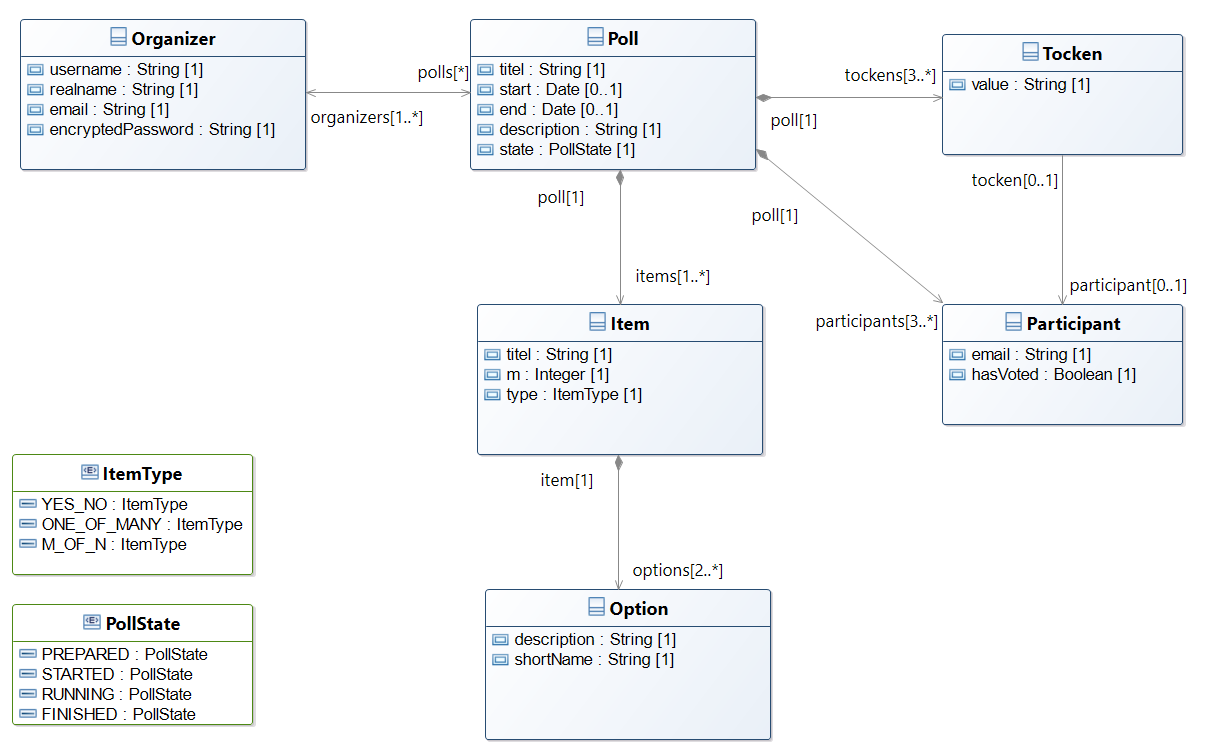
\includegraphics[width=1.0\textwidth]{png/domain_model.png}
\caption{Votes content model}
\end{figure}


\subsection{Navigation model}
% Maybe we can call that navigation model? Enables refference on http://uwe.pst.ifi.lmu.de/teachingTutorialNavigation.html
%Mentioned by ebert in the last web engeneering course! Will make rudige cum!

% I try it. Write mail if not ok! Max has to check that.
The navigation through the system and the interaction between user and content model is realised in html. The following model presented in figure \ref{navigation_model} focuses on the possible navigation paths. To define this on an abstract level we will coarsely stick to navigation model viewpoint defined by the UWE approve \cite{Uwe08,uweref}. It defines possible ways through the system by specifying different node types and one navigation links on the basis of UML stereotype. A node is the smallest unit where any user can navigate to. More than one node can be presented on a single web. Links are used to connect nodes and enable transitions, containment relations points out the structural containedness of one node in another.




\begin{figure}
\label{navigation_model}
\centering
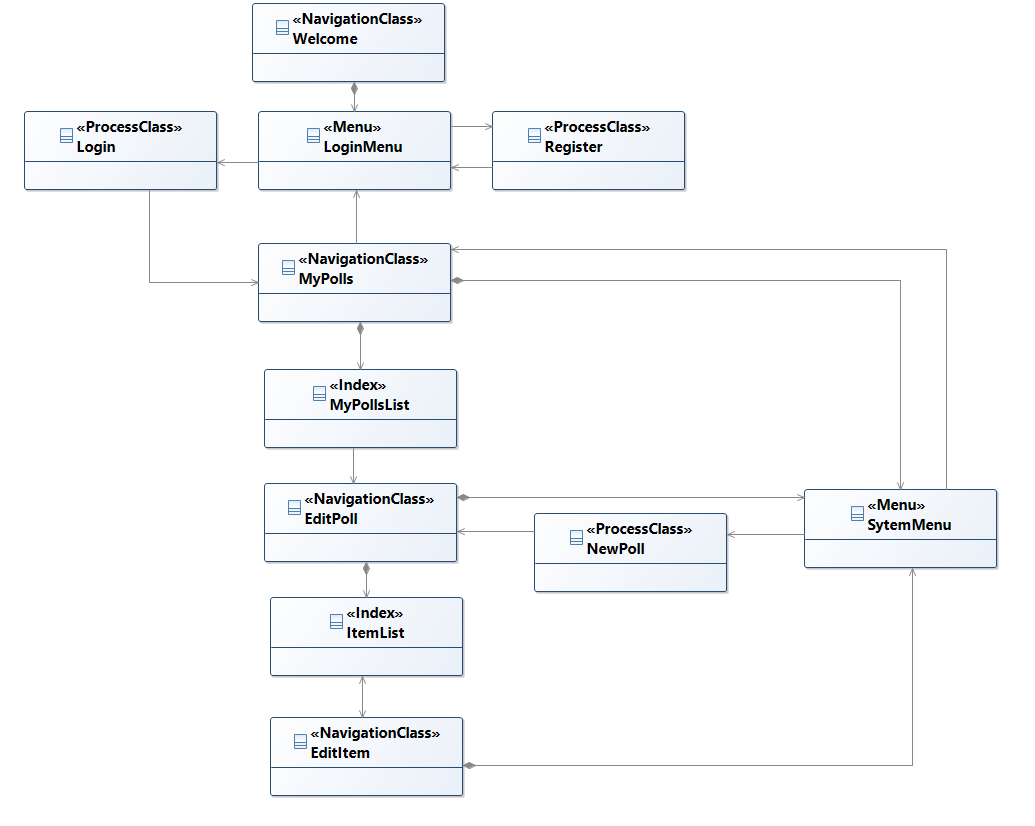
\includegraphics[width=1.0\textwidth]{png/navigation_model.png}
\caption{Votes navigation model}
\end{figure}

\subsection{Presentation model}
% If we insert the UWE Presentation model, i need help of max because i can not undesand html.

\subsection{VotesWar Architecture (Packaging?)}
% Do you mean packaging?